\chapter{Marco teórico y estado del arte}
\label{cap:MarcTeorico}

Este capítulo busca realizar una contextualización de los conceptos necesarios para entender el problema que se está tratando por medio de una breve reseña de cada uno. Además, se da a conocer la revisión de los trabajos existentes capaces de realizar tareas similares o basadas en principios similares a los planteados por la solución expuesta de este trabajo.

\section{Marco teórico}
\label{intro:motivacion:marco}

Se presentan las definiciones de herramientas y técnicas que sustentan a la solución implementada.

\subsection{Sistemas de procesamiento de \textit{streams}}
\label{subsec:SPS}

El sistema tradicional de procesamiento, el trabajo por lotes (\textit{batch}), está pensado en que primero los datos son recopilados y almacenados, para luego pasar a ser procesados. Sin embargo, este enfoque introduce una alta latencia en la obtención del resultado deseado, lo que no es útil en casos en que es necesario obtener resultados en tiempo real.

Para realizar este tipo de procesamiento en tiempo real existe otro enfoque, el procesamiento de \textit{streams}, el cual está diseñado para trabajar con datos que llegan al sistema directamente desde la fuente y en gran cantidad y son procesados uno por uno.

Un sistema de procesamiento de \textit{streams} se caracteriza, principalmente, por lo siguiente:

\begin{itemize}
\item Opera en memoria: procesamiento contínuo en flujos de datos en series de tiempo.
\item Escalable: arquitectura optimizada para latencia cercana a cero en grandes volúmenes de datos.
\item Escalabilidad a través de la distribución eficiente en múltiples procesadores o servidores.
\end{itemize}

Su funcionamiento es caracterizado por datos llegando de manera continua a los cuales se les aplica una o más operaciones las cuales pueden filtrar, agregar information, o transformar los datos entrantes.

Conceptualmente su arquitectura es un grafo de operaciones que se comunican entre ellas intercambiando flujos de datos, representados como flechas, y donde los nodos realizan tareas las cuales transforman esos datos para solucionar un problema. La Figura \ref{fig:ArqSPS} presenta cómo es una típica arquitectura de estos sistemas con los elementos antes mencionados, \citep{SPExplained}.

\begin{figure}[H]
	\centering
	\captionsetup{justification=centering}
	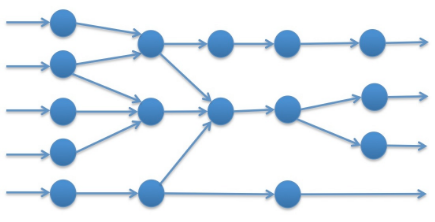
\includegraphics[scale=0.8]{images/ArqSPS.png}
	\caption[Arquitectura típica de sistemas de procesamiento de \textit{streams}.]{Arquitectura típica de sistemas de procesamiento de \textit{streams}.\\Fuente: \citep{SPExplained}}
	\label{fig:ArqSPS}
\end{figure}

Estos sistemas se enfrentan a en entorno cuyas características como por ejemplo, la cantidad de información que reciben, la cantidad que son capaces hacer fluir por ellos o \textit{throughput} y el tiempo que demoran en ello (latencia) presentan dificultades a la hora de pensar en sistemas de procesamiento en tiempo real.

Existen variados motores de procesamiento de \textit{streams}, sólo por mencionar algunos de ellos: S4 \citep{NeumeyerS4}, \textit{StreamCloud} \citep{GulisanoStreamCloud}, ESC \citep{SatzgerESC}, \textit{TimeStream} \citep{QianTimeStream}, T-Storm \citep{XuTStorm}, MillWheel \citep{AkidauMillWheel}, Storm \citep{StormFigure}.


\subsection{Minería de texto}
\label{subsec:MineriaTexto}

La minería de textos o \textit{text mining} es una rama de la lingüística computacional que trata de obtener información y conocimiento a partir de conjuntos de datos que en principio no tienen un orden o no están dispuestos en origen para transmitir esa informacion, \citep{IvanFernandez}. Para explicar este concepto, primero se introduce el concepto de minería de datos o \textit{data mining}.

\subsubsection*{Minería de datos}
\label{subsubsec:dataMining}

Para la minería de datos los datos son la materia prima, ésta se convierte en información que posteriormente es tratada y utilizada para convertirla en conocimiento. Reune áreas como la estadística, inteligencia artificial, bases de datos, y procesamiento masivo. \citep{LuisMolina} la define como ``\textit{la integración de un conjunto de áreas que tienen como propósito la identificación de un conocimiento obtenido a partir de las bases de datos que aporten un sesgo hacia la toma de decisión}".

La principal diferencia de la minería de datos con respecto a la minería de textos es que la primera utiliza bases de datos como materia prima, mientras la segunda hace uso de documentos para ello.

Una de las aplicaciones de la minería de textos es la clasificación de documentos. Esta práctica consiste en el uso de técnicas de aprendizaje automático para asignar categorías a un determinado texto, para ello existen algoritmos de clasificación con los cuales pueden construirse clasificadores capaces de agrupar eventos en categorias pre-establecidas.

\subsubsection*{Clasificadores}
\label{subsubsec:Classifiers}

En el campo del procesamiento de lenguaje natural el detectar patrones es una parte central. La clasificación es la tarea de seleccionar la etiqueta correcta para una entrada dada. Cada entrada es considerada como aislada de las demás, y el conjunto de etiquetas (o categorías), es definido con anterioridad.

Un clasificador es llamado ``supervisado" si ha sido construido a partir de un conjunto de datos de entrenamiento o \textit{corpus} de entrenamiento. La Figura \ref{fig:NPLK} muestra el proceso de entrenamiento y uso de un clasificador. (a) Durante el entrenamiento, un extractor de características es utilizado para convertir cada entrada a un conjunto de características, estos capturan la información básica de cada conjunto de entrada que es usada para clasificar. Pares de estos conjuntos y etiquetas son la entrada para el algoritmo que contruye el modelo de clasificación. (b) Durante la predicción se realiza el mismo procedimiento, pero sin entregar como entrada la etiqueta correspondiente, se pasa al modelo generado para obtener su predicción sobre la pertenencia a una etiqueta.

\begin{figure}[H]
	\centering
	\captionsetup{justification=centering}
	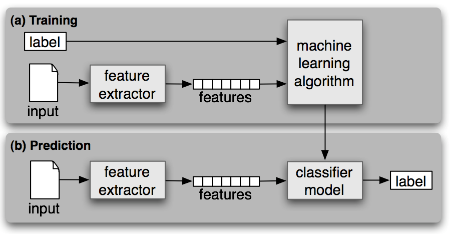
\includegraphics[scale=0.8]{images/TrainingPrediction.png}
	\caption[Clasificación supervisada en general.]{Clasificación supervisada en general.\\Fuente: \citep{NPLK}}
	\label{fig:NPLK}
\end{figure}

El modelo de clasificación construido debe evaluarse para decidir si es preciso. Para ello se requiere un conjunto de datos de evaluación que generalmente corresponden a un subconjunto entrada. El conjunto de entrenamiento se separa en dos categorías: los datos de entrenamiento y los datos de evaluación. Comúnmente, se utiliza un 10\% del conjunto total para formar los datos de evaluación, \citep{NPLK}.

La métrica más simple para evaluar un clasificador es la precisión (\textit{accuracy}), la cual corresponde la razón de entradas clasificadas correctamente. Matemáticamente:

\[
	Accuracy = \frac{TP}{TP+FP}
\]

TP y FP corresponden respectivamente a valores correctamente clasificados (\textit{true positives}) y valores clasificados incorrectamente (\textit{false positives}), también conocidos como ``Errores tipo I". Adicionalmente, existen otras dos métricas: TN y FN que, respectivamente corresponden a valores correctamente no clasificados como elementos de una etiqueta específica (\textit{true negatives}) y los conocidos como ``Errores tipo II", valores que no pertenecen a una etiqueta y han sido clasificados como tales (\textit{false negatives}). Con estos valores se pueden obtener dos nuevas métricas: El \textit{recall} y el medida F (\textit{F-Score}).

El \textit{recall}, indica el ratio de elementos clasificados correctamente y matemáticamente se define como sigue:

\[
	Recall = \frac{TP}{TP+FN}
\]

Por otro lado, la medida F combina precisión y \textit{recall} para entregar un puntaje, dado por la siguiente función:

\[
	F_{\beta} = (1+\beta^{2})\frac{Accuracy · Recall}{(\beta^{2} · Accuracy) + Recall}
\]

Típicamente se utiliza la medida armónica donde $\beta$ toma el valor 1, quedando la función como sigue:

\[
	F1 = 2\frac{Accuracy · Recall}{ Accuracy + Recall}
\]

Se dice que es la medida armónica, pues pondera de igual manera ambas razones, \citep{FMeasureInterpret}.

Existen diferentes métodos de aprendizaje de máquina utilizados para construir clasificadores, entre ellos están: \textit{Naïve Bayes}, máxima entropía y árboles de decisión.

Los árboles de decisión corresponden a un diagrama de flujo con el que se decide la etiqueta para una entrada. Los diagramas de flujo consisten en nodos de decisión, los que comprueban los conjuntos de características y las hojas que asignan las etiquetas. El más simple de ellos es llamado un \textit{decision stump}, el cual consiste en sólo un nodo de decisión y múltiples hojas, para construirlo se desarrollan todas las posibles etiquetas y se calcula la precisión para quedarse con aquellos que alcancen la más alta. Entonces, para construir un árbol de decisión con mayor nivel de generalización se van construyendo múltiples \textit{decision stumps} y usando aquellos con más alta probabilidad.

Para el caso de los clasificadores \textit{Naïve Bayes}, \citep{NaiveBayes2}, cada elemento del vector de características aporta en la determinación de qué etiqueta ha de ser utilizada. Para cada etiqueta se calcula su probabilidad \textit{a priori}, utilizando como referencia su frencuencia en el conjunto de entrenamiento. Esta probabilidad en conjunto con el aporte de cada elemento del vector determina una probabilidad de pertenencia, se le asigna a la entrada la etiqueta que tenga mayor probabilidad de pertenencia.

Los clasificadores máxima entropía, son similares a los clasificadores bayesianos, pero en lugar de utilizar las probabilidades establecer los parámetros del modelo, utilizan técnicas de búsqueda para encontrar parámetros que maximicen el desempeño del clasificador mediante técnicas de optimización iterativa, las que inician los parámetros en valores aleatorios y los refina mientras se va acercando al óptimo. Su principal desventaja es que toman mucho tiempo en realizar el aprendizaje dado el uso de las técnicas antes mencionadas, \citep{NPLK}.

Existen herramientas que contienen implementaciones de estos algoritmos, entre otros, y permiten generar clasificadores de manera más fácil y rápida. Se puede mencionar como ejemplo \citep{Weka}, acrónimo del inglés \textit{Waikato Envoirment for Knowledge Analysis}, RapidMiner \citep{RapidMiner} y Mallet \citep{Mallet}, acrónimo del inglés \textit{MAchine Learning for LanguagE Toolkit}.

En este trabajo se ha utilizado Mallet, herramienta desarrollada por \citep{Mallet}, en la Universidad de Massachusetts Amherst, La herramienta se encuentra en lenguaje Java y realiza procesamiento de lenguaje natural, clasificación de documentos, \textit{clustering}, extracción de información y otras aplicaciones de aprendizaje de máquina sobre texto. Mallet cuenta con implementaciones de una variedad de algoritmos entre los cuales se encuentran: \textit{Naïve Bayes}, máxima entropía y árboles de decisión. Además, incluye herramientas para evaluar el desempeño de clasificadores mediante el uso de métricas más utilizadas.

\subsection{Bases de datos no relacionales}
\label{subsubsec:BDNoSQL}

Las bases de datos no relacionales se separan de los principios expresados por \citep{CoddSQL}, pues no utilizan el lenguaje SQL, prácticamente universal en las bases de datos convencionales. Estas últimas organizan la información en tablas, cada una de ellas tiene un número de columnas o campos especificados por el administrador y  filas correspondiente a los datos. Además, estas tablas pueden relacionarse entre sí con relaciones uno a uno entre los elementos o uno a varios, de manera que mediante consultas que combinan varias tablas pueden obtener información de varias de ellas, estas consultas se realizan mediante un sencillo lenguaje estandarizado.

Las bases de datos tradicionales están diseñadas para mantener la integridad de las relaciones, por ejemplo: una tabla ``alumnos" está relacionada con la tabla ``calificaciones" y no pueden haber calificaciones para un alumno inexistente. 

El problema del modelo antes mencionado está en que son costosas en términos de rendimiento, dadas las garantías ofrecidas sobre los datos y transacciones. Lo que no es problema en lugares donde la información es limitada y se realizan pocas escrituras, pues éstas son caras computacionalmente. El verdadero problema está cuando la cantidad de información es muy grande, donde el uso de bases de datos relacionales obliga a dedicar mucho esfuerzo a la optimización para obtener un resultado aceptable.

Aproximándose a lo no relacional se renuncia a las tablas perfectamente definidas, que garantizan la integridad y donde todo parece predecible, pero se obtiene rapidez y flexibilidad. En el sistema de gestión de base de datos no relacionales como \citep{CassandraNOSQL}, \citep{redisNOSQL}, \citep{MongoDB}, toda la información está en el mismo sitio. Al acceder a los datos de un alumno, siguiendo la línea del ejemplo anterior, toda estará ahí, incluidas sus calificaciones y no existe información relacional, \citep{BDNOSQL}.

El caso de MongoDB, corresponde es una base de datos no relacional (NoSQL), de código abierto escrita en C++ y orientada al trabajo en documentos. Lo anterior quiere decir que en lugar de guardar los datos en tablas, lo hace en documentos, los que son almacenados como una representación binaria de JSON conocida como BSON.

Una de las diferencias fundamentales con respecto a las bases de datos relacionales es que no es necesario que se siga un esquema; en una misma colección — concepto similar a una tabla en las bases de datos relacionales — se pueden tener distintos esquemas.

MongoDB fue creado para brindar escalabilidad, rendimiento y disponibilidad. Puede ser utilizado en un servidor único como en múltiples. Esto se logra dado que MongoDB brinda un elevado rendimiento, tanto para lectura como para escritura, potenciando la computación en memoria, \citep{MongoDB}.

En pruebas realizando operaciones habituales dentro de las bases de datos, \citep{MongoPerformance}, demostró que el tiempo de ejecución de MongoDB, como base de datos NoSQL, aventaja significativamente a las bases de datos relacionales más populares como lo son MySQL y PostgreSQL.

\section{Estado del arte}
\label{intro:motivacion:arte}

El problema a abordar consta de tres tópicos centrales: plataformas orientadas a desastres, plataformas de procesamiento escalable y herramientas para la clasificación de eventos. La presente sección aborda los trabajos relacionados con la aplicación que se desea construir en las tres temáticas anteriormente menciondas.

\subsection{Plataformas de procesamiento para desastres}
\label{arte:PPDesastres}

El \textit{Qatar Computing Research Institute} \footnote{http://qcri.com}, es líder a nivel mundial en la creación de herramientas para dar soporte a desastres naturales usando tecnologías de la información, colaborando con grandes organizaciones como Naciones Unidas, Cruz Roja Internacional y UNICEF. Recientemente, han elaborado distintas aplicaciones (\textit{MicroMappers}, \textit{AIDR}, \textit{UAViators}, etc.), para ayudar a darle sentido al gran flujo de información que reciben los centros de ayuda humanitaria (\textit{Big crisis data}), generada por redes sociales, SMS, imágenes satelitales y aéreas tomadas por drones, que de otra forma serían incapaces de analizar.
Tomando la información, estas aplicaciones unen la ayuda de voluntarios y profesionales digitales, quienes están dispuestos a colaborar a través de Internet realizando tareas como identificación o clasificación. Con ésta y el poder del aprendizaje de máquina, se entrenan algoritmos para analizar millones de datos.

\textit{Micromappers} \citep{MicroMappers} es una aplicación creada por \textit{Qatar Computing Research Institute}, que permite a voluntarios digitales etiquetar diferente tipos de información para la ayuda en el proceso de respuesta a desastres y desplegarlos en un mapa. En el caso del terremoto de Nepal por ejemplo, los voluntarios han contribuido revisando miles de \textit{tweets} e imágenes para entregar una evaluación de impacto que ayuda a la toma de decisiones. La evolución de esta herramienta está orientada a integrarse con \textit{AIDR} para que la información obtenida de las personas a través de \textit{crowdsourcing} pueda servir para la automatización de proceso de clasificación mediante aprendizaje de máquina, y así subir al análisis de miles a millones de datos generados en situaciones de emergencia. Esta plataforma, a diferencia de lo propuesto en el presente trabajo, es una plataforma genérica de procesamiento de datos de crisis o desastres que no aborda el proceso de detección de necesidades, sino más bien, organizar la información que se genera en las diferentes fuentes de datos utilizada.

\textit{AIDR} (\textit{Artificial Intelligence for Disaster Response}), \citep{AIDR}, delega al aprendizaje de máquina la identificación de contenido durante desastres en \textit{Twitter}. Va más allá de un simple filtro por palabras clave que limitan la búsqueda a ellas y al lenguaje. textit{AIDR} está compuesto de tres partes: el colector, el entrenador y el etiquetador. El primero recolecta y almacena los datos, el entrenador construye un etiquetador automático y permite a usuarios realizar esto dado un conjunto de \textit{tweets} capturados por el colector, el etiquetador analiza los \textit{tweets} clasificados por humanos para automáticamente etiquetar nuevos \textit{tweets}. Esta plataforma no considera un sistema de procesamiento de \textit{streams}, de manera general, plantea una plataforma orientada a cómo generar sistemas automáticos de clasificación de eventos.

\textit{UAViators} \citep{UAViators}, iniciativa también creada por \textit{Qatar Computing Research Institute}, reúne información generada por drones que entregan imágenes para crear conocimiento sobre el área del desastre en tiempo real. Su procesamiento puede entregar información como una estimación de la población afectada, daños en infraestructura de edificios, líneas de electricidad, carreteras, campamentos base, entre otros. Esta plataforma posee un objetivo muy diferente al planteado por la solución propuesta en esta memoria, sin embargo ambas soluciones pueden ser complementarias.

\subsection{Procesamiento de datos a gran escala}
\label{arte:SPS}

En los últimos años, un nuevo paradigma de procesamiento se sumó al ya conocido esquema \textit{map-reduce}. Este nuevo paradigma, a diferencia del anteriormente mencionado, es capaz de procesar información \textit{online} sin requerir de un almacenamiento previo de los datos. Este esquema se adapta de mejor manera la tendencia de extraer conocimiento de las interacciones \textit{online} de los usuarios. A continuación se presentan algunas de las implementaciones de estos paradigmas de procesamiento.

\subsubsection*{\textit{MapReduce}}
\label{arte:SPS:mapreduce}

El \textit{framework} de Google \textit{MapReduce}, \citep{DeanMapReduce}, es un modelo de programación diseñado para procesar conjuntos de datos a gran escala en una modalidad orientada al lote (\textit{batch}). Este sistema está orientado a programación funcional y utiliza funciones del tipo \textit{map} y \textit{reduce}. \textit{MapReduce} ha logrado gran popularidad en aplicaciones orientadas a grandes volúmenes de datos dado su modelo de programación basado en clave/valor y su escalabilidad. Las soluciones presentadas en \citep{CondieMapReduce} y \citep{VermaMapReduce}, están orientadas al procesamiento de flujos de datos en línea basadas en \textit{MapReduce}. \citep{CondieMapReduce} proponen modificaciones a \textit{Hadoop}, que es una implementación de \textit{MapReduce} de código abierto, y que permite que los datos sean canalizados entre los operadores haciéndolo más adecuado a aplicaciones con requerimientos de tiempo real. 

\subsubsection*{Apache S4}
\label{arte:SPS:s4}
					
S4, \citep{NeumeyerS4}, o \textit{Simple Scalable Streaming System} es un sistema de propósito general, distribuido y escalable que permite que aplicaciones puedan procesar flujos de datos de forma continua y sin restricciones. S4 está inspirado en \textit{MapReduce} y fue diseñado en el contexto de minería de datos y algoritmos de aprendizaje de máquina en \textit{Yahoo! Labs} para sistemas de publicidad \textit{online}. Cada evento en S4 es descrito como un par (clave, atributo). La unidad básica son los elementos de procesamiento (PEs) y los mensajes que son intercambiados entre ellos. Los PEs pueden emitir o pueden publicar resultados y son alojados en servidores llamados nodos de procesamiento (PNs). Los PNs son responsables de escuchar eventos, rutear eventos a los PEs del nodo y despachar eventos a través de la capa de comunicación. Los eventos son encaminados usando una función de \textit{hashing} sobre los valores de los atributos hacia el PE apropiado. Por otro lado, la capa de comunicación utiliza Zookeeper, \citep{HuntZookeeper}, que provee manejo de clusters y reemplazo automático de nodos que fallan. S4 usa encaminamiento estático, es parcialmente tolerante a fallas, y no posee mecanismos de balanceo dinámico de carga.
					
Actualmente, S4 está en fase de incubación en la fundación Apache, pero no ha tenido avances en el proyecto desde el junio del año 2013, cuando se lanzó su versión 0.6.0.

\subsubsection*{Apache Spark}
\label{arte:SPS:spark}

\textit{Spark}, \citep{SparkOnline}, es una plataforma de computación de código abierto para análisis y procesos avanzados, que tiene muchas ventajas sobre \textit{Hadoop}. Desde el principio, \textit{Spark} fue diseñado para soportar en memoria algoritmos iterativos que se pudiesen desarrollar sin escribir un conjunto de resultados cada vez que se procesaba un dato. Esta habilidad para mantener todo en memoria es una técnica de computación de alto rendimiento aplicado al análisis avanzado, la cual permite que \textit{Spark} tenga unas velocidades de procesamiento que puedan ser hasta 100 veces más rápidas que las conseguidas utilizando \textit{MapReduce}, \citep{Spark}.

\subsubsection*{Apache Storm}
\label{arte:SPS:storm}
					
\textit{Apache Storm} es una plataforma similar a S4, está implementado como una API para la computación \textit{streams} de datos en tiempo real desde una o múltiples fuentes de manera distribuida, tolerante a fallos y de alta disponibilidad. \textit{Storm} está principalmente pensado para trabajar con datos que deben ser analizados en tiempo real, \citep{Storm}.

\textit{Apache Storm} es escalable y garantiza que toda la información será procesada. Presenta \textit{benchmarks} que señalan que por nodo es capaz de procesar más de un millón de tuplas por segundo.

Un sistema construido haciendo uso de \textit{Storm} está compuesto por elementos procesadores de dos tipos: el primero es denominado \textit{spout} y es el encargado de recoger el flujo de datos de entrada. El segundo es denominado \textit{bolt} y es el encargado de la transformación o procesado de los datos, para una transformación compleja se requiere mayor número de \textit{bolts}.

Una aplicación realizada en \textit{Storm} es representada como puede verse en la Figura \ref{fig:stormBeLike}, donde los \textit{spouts} son representados simulando ser llaves de agua desde donde fluyen los datos al sistema y los \textit{bolts} como rayos donde se procesa el flujo.

\begin{figure}[H]
	\centering
	\captionsetup{justification=centering}
	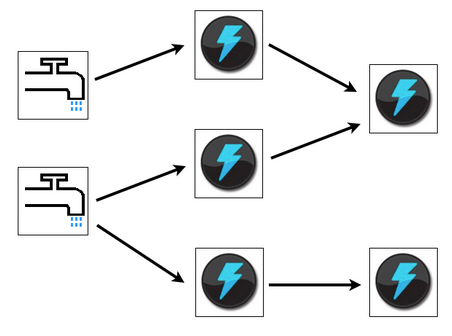
\includegraphics[scale=0.6]{images/stormBeLike.png}
	\caption[Representación del funcionamiento de Apache Storm.]{Representación del funcionamiento de Apache Storm.\\Fuente: \citep{StormFigure}}
	\label{fig:stormBeLike}
\end{figure}

Uno de los puntos fuertes que tiene este sistema, y que está en línea con lo señalado para sistemas de procesamiento de \textit{stream}, es que al crear una topología donde se instancian \textit{bolts} y \textit{spouts}, \textit{Storm} se encarga de escalar el sistema distribuyendo los elementos en sus componentes. Una topología de \textit{Storm} corresponde, en su nivel más alto de abstracción, a un grafo acíclico dirigido, \citep{Storm}.

\textit{Storm} tiene diferentes modos de funcionamiento, referido a la forma en la que se van a compartir los datos entre los componentes. Como modelo de datos, \textit{Storm} utiliza tuplas que son listas de valores con un nombre asociado, \citep{Storm}, las cuales pueden ser enviadas al siguiente nodo de las siguientes formas:

\begin{itemize}
\item \textit{Shuffle grouping}: \textit{Storm} decide de forma \textit{round robin} la tarea a la que se va a enviar la tupla, de manera que la distribución sea equivalente entre todos los nodos.
\item \textit{Fields grouping}: se agrupan los \textit{streams} por un determinado campo de manera que se distribuyen los valores que cumplen una determinada condición a la misma tarea.
\item \textit{All grouping}: el \textit{stream} pasa por todas las tareas haciendo multicast.
\item \textit{Grobal grouping}: el \textit{stream} se envía al \textit{bolt} con ID más bajo.
\item \textit{None grouping}: es un \textit{Shuffle grouping} donde el orden no es importante.
\item \textit{Direct grouping}: la tarea es la encargada de decidir hacia donde emitir especificando el ID del destinatario.
\item \textit{Local grouping}: se utiliza el mismo \textit{bolt} si tiene una o más tareas en el mismo proceso.
\end{itemize}

\textit{Storm} puede funcionar de dos modos: local y \textit{cluster}. El primero es útil para el desarrollo, pues ejecuta toda la topología en una única máquina virtual de Java (JVM), por lo que pueden realizarse fácilmente pruebas de integración, como por ejemplo depurar código. Este modo simula cada nodo del \textit{cluster} haciendo uso de \textit{threads}, \citep{Storm}. El modo \textit{cluster} es considerado el ``modo de producción" y es el modo donde el código es distribuido en máquinas diferentes dentro del \textit{cluster}.

La arquitectura de Storm se divide en tres componentes:

\begin{itemize}
\item \textit{Master Node}: ejecuta el demonio llamado \textit{Nimbus}, el cual es responsable de distribuir el código a través del \textit{cluster}. Realiza la asignación y monitorización de tareas en las distintas máquinas del cluster.
\item \textit{Worker Node}: ejecutan el demonio \textit{Supervisor}, el cual se encarga de recoger y procesar los trabajos asignados en la máquina donde está siendo ejecutado. En caso de fallo de uno \textit{Worker Node}, \textit{Nimbus} redirige el trabajo a otro nodo.
\item \textit{Zookeeper}: si bien no es un componente propio de \textit{Storm}, es necesario para su funcionamiento, pues se encarga de coordinar \textit{Nimbus} y \textit{Supervisor} dado que estos no guardan su estado, \textit{Zookeeper} lo hace por ellos, \citep{StormState}.
\end{itemize}	

\subsection{Clasificación de eventos}
\label{intro:ea:clasificacion}

La clasificación de texto en servicios de \textit{microblogging}, como \textit{Twitter} es un problema cuya solución tiene diferentes puntos de vista, los métodos tradicionales incluyen hacer uso de una bolsa de palabras para clasificar según el contenido del texto, construcción de n-gramas para clasificar según términos co-ocurrentes o ubicar el texto en una categoría haciendo uso de técnicas de aprendizaje de máquina o \textit{Machine Learning}, \citep{EventDetection}. 
Este último método ya ha sido comprobado por diversos autores, entre ellos \citep{Maldonado}, quien utilizó este método para realizar su memoria donde clasificaba \textit{tweets} según sentimientos encontrados en el texto, los cuales se clasificaban como positivos, negativos o neutros. Para ello hizo uso de un clasificador \textit{Naïve Bayes} y \textit{Support Vector Machine} (SVM). 

En el marco de las jornadas chilenas de la computación \citep{WladdimiroPMI}, propusieron un modelo desarrollado para el proyecto PMI USA 1204: Despliegue ágil de aplicaciones para desastres \citep{PMIProfes}, donde analizaron el rendimiento de una aplicación de clasificación de necesidades básica al ser implementada en un sistema de procesamiento de \textit{streams} como S4. En él se propone un modelo basado en \textit{Yahoo! S4} donde, haciendo uso del paradigma de procesamiento de \textit{streams} de datos, se forma un grafo cuyos nodos (Elementos de procesamiento o PE, por sus siglas en inglés) dividen el procesamiento en pequeñas tareas fácilmente replicables para paralelizar el \textit{pipeline}. En esa ocación desarrollaron distintos tipos de operadores mencionados a continuación:

\begin{itemize}
\item Recolector: haciedo uso de la API de \textit{Twitter} obtiene el \textit{stream} de datos del mismo. 
\item \textit{Scheduler}: discrimina cada \textit{tweet} según la categoría a la que pertenece (información, agua, electricidad o alimento), mediante el uso de una bolsa de palabras y la distancia \textit{Hamming}.
\item Filtrado: utilizaron en su trabajo un clasificador basado en \textit{machine learning} para verificar la subjetividad de un \textit{tweet}, por lo que ya esta demostrado que esta herramienta es capaz de categorizar texto, por lo que puede ser aplicada para las entradas de \textit{Twitter}.
\item Relevancia: identificar si una información es o no confiable haciendo uso de la cantidad de publicaciones del usuario, sus seguidores y a quienes sigue para estimar una reputación del autor.
\item Ranking: hace uso de la información anterior, decidiendo a que \textit{tweet} le entrega mayor importancia.
\end{itemize}

Los autores concluyeron sobre la importancia de una replicación adecuada para distribuir la carga entre los operadores basándose en la carga computacional, pero no fueron concluyentes en cuánto o qué nivel de replicación es el adecuado o cuándo replicar.

A modo de comentario se señala que diversos autores, entre los que se puede mencionar a \citep{VanDeVoort}, \citep{EventDetectionInTwitter}, \citep{Maldonado}, han señalado las dificultades que se presentan al trabajar utilizando como entradas los estados públicos (\textit{tweet}) de los usuarios de \textit{Twitter}. Dentro de las dificultades señaladas se encuentran, por ejemplo, el acceso a la información; si bien existen accesos públicos a la información estos son restringidos tanto en cantidad como en tiempo. Este punto de acceso permite acceder a un 1\% de la información generada en un instante, es decir, por cada cien \textit{tweets} generados en la red \textit{Twitter} sólo 1 es emitido de manera pública a la API. Además, existe una restricción a la cantidad de elementos que pueden ser obtenidos en un intervalo de tiempo, luego de que este límite es alcanzado, se ha de esperar para volver a acceder a los datos del \textit{stream}. Si se desea trabajar sin estas limitaciones, se puede hacer uso del llamado \textit{FireHose} de \textit{Twitter}, el cual entrega todo el flujo de eventos generados en la red sin limitaciones, sin embargo esta modalidad es de pago.

Por otro lado, \citep{VanDeVoort} señala que la dificultad radica en el hecho de que cualquier persona puede realizar publicaciones en esta red social induciendo ruido en la información (considerando el ruido como toda información que aparece junto a la deseada, pero no aporta nueva información), además de que, al ser publicaciones de máximo 140 caracteres es complejo contextualizar el contenido.

--- AGREGAR CONCLUSION DE CIERRE DEL CAP ---
